\chapter{Experimental Design}

\section{Materials and Methods}
\subsection{Materials}
The experimental setup requires the following equipment and materials:
\begin{itemize}
\item GelMA premix solution
\item Custom 3D printer with syringe-based extruder
\item Load cell
\item Computer
\item Measuring tape
\item Digital vernier caliper
\end{itemize}

The bioprinter is made up of an extruder, gantry, and curing system. A UV source is used to irradiate the GelMA prints to induce curing. The extruder uses a leadscrew to extrude the GelMA out of a syringe (onto a glass bed) that is wrapped in alumium foil (to prevent premature curing), and the force is measured using a load cell and sampled using an STM32 microcontroller. The extruder position is varied with a gantry that uses belts to adjust the extruder position along the horizontal plain and uses a lead screw to adjust the nozzle offset.

The bioprinter’s printing parameters are adjusted using a computer which behaves as an interface and the prints produced in each trial of the experiment are measured using a measuring tape and digital vernier caliper. This experimental setup is shown below in Figure~\ref{fig:experimentalSetup}:
 \begin{figure}[h]
    \centering
    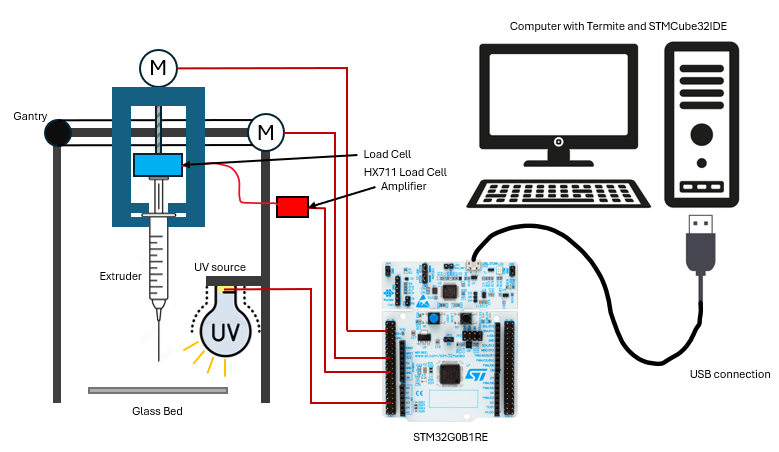
\includegraphics[scale=0.7]{figs/ExperimentalSetup.png}
    \caption{Experimental Setup (please change pic)}
    \label{fig:experimentalSetup}
\end{figure}

\subsection{Equipment Specifications}
The experimental equipment needs to allow a 10mm line of GelMA to be extruded onto a printing bed where the print line’s width and can be measured at points along the line without distorting the print line’s dimensions over the course of the measurement process as this would decrease the reliability of the measurements. The experiment also needs a way to configure the bioprinter’s parameters and receive real time printing feedback.


\subsubsection*{GelMA Specifications}

The Gelatin Methacrylate premix solution consists of GelMA and Irgacure 2959 (a photoinitiator that gives the solution its curing ability), which are dissolved in a solvent known as Phosphate Buffered Saline (PBS). The final composition is 10\% w/v GelMA with 0.1\% w/v Irgacure 2959 in PBS. The GelMA premix must be stored at 4\,\textdegree{}C, protected from UV light (to prevent premature curing) by wrapping its container in aluminium foil, and used to print within 2 weeks of preparation \citep{gelma_protocol}.

\subsubsection*{Bioprinter Specifications}

\begin{itemize}
    \item \textbf{Load cell} – A 50\,kg load cell is mounted to the extruder and is used with an HX711 load cell amplifier, which conditions the signal and sends it to the printer’s controller (STM32G0B1RE) via a digital output and clock terminal. The purpose of the load cell is to provide real-time measurement (through Termite) of the extrusion force to monitor for extrusion risks such as clogging, which is identified by irregularly high extrusion forces.
    
    \item \textbf{Extruder} – This consists of a syringe with a volume of 10\,ml and a nozzle diameter of 1\,mm. A leadscrew with a 2\,mm pitch is driven by a NEMA 17 stepper motor to extrude the GelMA out of the syringe.
    
    \item \textbf{Gantry} – The gantry is used to position the extruder in 3D space. Two NEMA 17 stepper motors drive belts that control the 2-axis motion in the horizontal plane. A leadscrew (also driven by a NEMA 17) with a 2\,mm pitch is used to control the extruder’s vertical position.
    
    \item \textbf{Bed} – The GelMA is printed on a 15\,mm $\times$ 15\,mm glass bed.
    
    \item \textbf{Curing system} – This comprises a UV LED that shines ultraviolet light with a wavelength of 365\,nm for 5 minutes after printing \cite{gelma_protocol}, ensuring the size and shape of the print remains stable and does not change during measurement.
\end{itemize}

\subsubsection*{Software}

\begin{itemize}
    \item \textbf{STM32CubeIDE} – The IDE is used to configure the printing parameters by adjusting the code that the STM32G0B1RE runs.

    \item \textbf{Termite} – The STM32G0B1RE sends real-time measurement data of the extruder position, bed temperature, and extrusion force via UART communication. This data is received and displayed by Termite through a USB cable. This is useful for real-time monitoring of each print and ensures smooth operation of the bioprinter.

    \item \textbf{MATLAB} – The data obtained from manually measuring the print width and height can be processed and plotted using MATLAB.
\end{itemize}


\subsection{Methods}
The variables identified in this experiment are shown below in Table~\ref{tab:variables}:
\begin{longtable}{|>{\raggedright\arraybackslash}p{4cm}|>{\raggedright\arraybackslash}p{10cm}|}
\caption{Experimental Variables} \label{tab:variables} \\
\hline
\textbf{Variable Type} & \textbf{Variables} \\
\hline
\endfirsthead

\hline
\textbf{Variable Type} & \textbf{Variables} \\
\hline
\endhead

Independent Variables & Extrusion rate, Printing speed, Nozzle height \\
Dependent Variables   & Extrusion force, Layer height, Layer width, Print quality \\
Controlled Variables  & GelMA concentration, Nozzle diameter \\
Extraneous Variables  & Ambient temperature, Vibrations \\
\hline
\end{longtable}


During the analysis of results, the mean layer height and width, as well as the standard deviation of the layer height and width (in mm) along each of the 10\,mm printed lines, are tabulated against the varied printing parameters: extrusion rate (mm/s), printing speed (mm/s), and nozzle height (mm). The two standard deviations serve as separate measures of print quality, where high deviations indicate lower print stability and quality.

The extrusion force from the load cell, measured via the COM port using MATLAB, is also plotted against time for each of the four different extrusion rates. The nozzle diameter affects both the speed and width of the extruded gel, influencing the resulting line width, height, and quality. These dependent variables are also affected by the rheological properties of the GelMA, which is why nozzle diameter and GelMA concentration are kept constant as controlled variables.

Ambient temperature and environmental vibrations, including those from the printer itself, can also influence outcomes. However, these are considered extraneous variables and are not within the scope of control in this experiment.

\subsubsection*{Experimental Setup Procedure}

Before the experiment can be conducted, the following setup procedure must be followed:

\begin{enumerate}
    \item Remove the GelMA premix from storage.
    \item Slowly load the GelMA premix solution into the syringe by fully submerging the syringe nozzle into the solution and pulling the plunger to minimize air bubbles in the loaded syringe. Air bubbles can compromise print quality by causing sudden breaks in the printed line.
    \item Allow the loaded syringe to sit for one hour to reach room temperature, reducing viscosity and aiding in air bubble removal. Then hold the syringe vertically with the nozzle facing upwards and flick the syringe to float any remaining bubbles to the top. Carefully push the plunger until hydrogel begins to extrude.
    \item Wrap the extruder in aluminium foil to prevent premature curing inside the syringe.
    \item Load the syringe into the bioprinter.
    \item Connect the printer to power.
    \item Use STM32CubeIDE and Termite to configure controller settings. Ensure the load cell reads zero and is scaled correctly using a known calibration weight.
    \item Connect the STM32G0B1RE to the computer via USB cable.
    \item Verify that both MATLAB and Termite are configured to read live data from the correct COM port.
\end{enumerate}

\subsubsection*{Test Procedure}

Once the setup is complete, the following test procedure is performed:

\begin{enumerate}
    \item Use STM32CubeIDE to vary the extrusion rate (mm/s), printing speed (mm/s), and nozzle offset (mm).
    \item Begin the extrusion process to deposit a 10\,mm long GelMA line onto the bed. Monitor the print using Termite.
    \item Use MATLAB to acquire and process the time-based extrusion force data for each extrusion rate.
    \item After printing, if no UV shielding is present, evacuate the room while the UV light cures the print for 5 minutes.
    \item Re-enter the room and measure the printed line’s width and height at 10 equidistant points (1\,mm apart) using a digital caliper.
    \item Record the mean and standard deviation of the 10 measurements for both width and height. These serve as metrics for print stability and quality.
    \item Repeat each test condition three times. Compute 95\% confidence intervals for each of the four measured variables (mean and standard deviation of width and height) to quantify measurement uncertainty and evaluate repeatability.
\end{enumerate}

A proposed test matrix is shown in Table~\ref{tab:testmatrix}, which outlines the combination of printing parameters for each trial in the experiment.

\begin{longtable}{ccc}
\caption{Proposed Test Matrix for Each Experiment} \label{tab:testmatrix} \\
\hline
\textbf{Test No.} & \textbf{Printing Speed (mm/s)} & \textbf{Extrusion Speed (mm/s)} \\
\hline
1  & 1 & 0.025 \\
2  & 1 & 0.050 \\
3  & 1 & 0.075 \\
4  & 1 & 0.100 \\
5  & 2 & 0.025 \\
6  & 2 & 0.050 \\
7  & 2 & 0.075 \\
8  & 2 & 0.100 \\
9  & 3 & 0.025 \\
10 & 3 & 0.050 \\
11 & 3 & 0.075 \\
12 & 3 & 0.100 \\
13 & 4 & 0.025 \\
14 & 4 & 0.050 \\
15 & 4 & 0.075 \\
16 & 4 & 0.100 \\
\hline
\end{longtable}
These tests are split up into two experiments, two compare the variation of nozzle offset. In experiment A, the nozzle offset is set to 2mm and in experiment B, it is set to 4mm.

\section{Discussion of Results and Conclusion}
Each test is iterated 3 times. This means that the 16 tests performed for each nozzle height (2 in total) will be iterated 3 times, yielding a total of 96 tests in total. The mean (across the 3 iterations) for the four measured variables per test will be calculated and tabulated in Table 3 below for each nozzle height.

{\small
\begin{longtable}{>{\raggedright\arraybackslash}p{1cm} 
                  >{\centering\arraybackslash}p{2cm} 
                  >{\centering\arraybackslash}p{2cm} 
                  >{\centering\arraybackslash}p{1.5cm} 
                  >{\centering\arraybackslash}p{1.5cm} 
                  >{\centering\arraybackslash}p{1.5cm}
                  >{\centering\arraybackslash}p{1.5cm}}
\caption{Results Table Template}  \label{tab:results} \\
\hline

\textbf{Test No.} & \textbf{Print Speed (mm/s)} & \textbf{Extrusion Speed (mm/s)} & \textbf{Mean Width (mm)} & \textbf{Mean Height (mm)} & \textbf{Std Dev Width (mm)} & \textbf{Std Dev Height (mm)} \\
\hline
\endhead
\hline
1  & 1 & 0.025 & -- & -- & -- & -- \\
2  & 1 & 0.050 & -- & -- & -- & -- \\
3  & 1 & 0.075 & -- & -- & -- & -- \\
4  & 1 & 0.100 & -- & -- & -- & -- \\
5  & 2 & 0.025 & -- & -- & -- & -- \\
6  & 2 & 0.050 & -- & -- & -- & -- \\
7  & 2 & 0.075 & -- & -- & -- & -- \\
8  & 2 & 0.100 & -- & -- & -- & -- \\
9  & 3 & 0.025 & -- & -- & -- & -- \\
10 & 3 & 0.050 & -- & -- & -- & -- \\
11 & 3 & 0.075 & -- & -- & -- & -- \\
12 & 3 & 0.100 & -- & -- & -- & -- \\
13 & 4 & 0.025 & -- & -- & -- & -- \\
14 & 4 & 0.050 & -- & -- & -- & -- \\
15 & 4 & 0.075 & -- & -- & -- & -- \\
16 & 4 & 0.100 & -- & -- & -- & -- \\
\hline
\end{longtable}
}


The tabulated data is used to determine the combination of print parameter for each printing speed that yields print lines with the best quality (lowest standard deviation of height and width). Confidence intervals for all 4 dependent variables, can be calculated from the three iterations.

These intervals will be tabulated in two more tables (identical to Table~\ref{tab:results}). They will be used to determine the uncertainty from random errors, which will be evaluated to determine the repeatable of the experiment.

After the uncertainty analysis, the extrusion force for each of the four extrusion rates can be plotted against time in seconds on a single plot using MATLAB. This may provide valuable information in characterising the rheological properties of the GelMA premix solution that can be used to determine new combinations of printing parameters for test matrices used in future versions of this experiment.

The successful completion of this experiment will produce a quantified relationship between print quality and the various printing parameters of the GelMA 3D bioprinter as well as provide information that will be useful for determining different print parameter ranges in future iterations of the experiment. The produced information will be used to produce more accurate and high-quality prints in the field of tissue engineering.